\documentclass[10pt]{article}
% TMLR submission (anonymized). Camera-ready: \usepackage[accepted]{tmlr}
\usepackage{tmlr}
\usepackage[T1]{fontenc}
\usepackage[utf8]{inputenc}
\usepackage{microtype}
\usepackage{amsmath,amssymb,amsthm}
\usepackage{booktabs}
\usepackage{tabularx}
\usepackage{enumitem}
\usepackage{xcolor}
\usepackage{tikz}
\usetikzlibrary{arrows.meta,positioning,fit,backgrounds}
\usepackage{pgfplots}
\pgfplotsset{compat=1.16}
\usepackage{url}
\usepackage[colorlinks=true,linkcolor=blue!50!black,citecolor=blue!50!black,urlcolor=blue!50!black]{hyperref}
\usepackage[capitalise,noabbrev]{cleveref}

\newtheorem{definition}{Definition}
\newtheorem{proposition}{Proposition}
\newtheorem{hypothesis}{Hypothesis}
\theoremstyle{remark}
\newtheorem{remark}{Remark}

\newcommand{\R}{\mathbb{R}}
\newcommand{\Sm}{\mathbf{S}}
\newcommand{\Cm}{\mathbf{C}}
\newcommand{\Hm}{\mathbf{H}}
\newcommand{\PS}{\textsuperscript{(P)}}
\newcommand{\IN}{\textsuperscript{(I)}}
\newcommand{\cdlr}{\textsc{CDLR}}

\title{Synaptic State or KV-Cache? A Unified Associative-Memory View, a Dual-Timescale Architecture Class, and a Matched-Compute Protocol}

% Anonymized for double-blind review; filled in only for camera-ready ([accepted] option).
\author{\name Jalendar Reddy Maligireddy \email jalendarreddy97@gmail.com \\
      \addr University of the Cumberlands}

\def\month{MM}
\def\year{YYYY}
\def\openreview{\url{https://openreview.net/forum?id=XXXX}}

\begin{document}
\maketitle

\begin{abstract}
Softmax attention stores context in a key--value cache that grows with sequence length; Hebbian ``synaptic''
models such as the Dragon Hatchling (BDH) store it in a fixed-size, positive, high-dimensional state rewritten at
every token; and recurrent latent reasoners such as BDH-CQ write demonstrations into such a state and then iterate
in latent space. We ask \emph{when, and at what cost, inference-time memory should be synaptic rather than a
cache}. We (i)~cast all three families as one associative-memory operator with explicit write, read, forgetting,
consolidation, and workspace maps, with byte accounting that yields a closed-form memory crossover $T^\star$;
(ii)~prove that any state with data-independent exponential forgetting couples retention and interference, so
no decay rate can both adapt quickly and retain earlier episodes; (iii)~specify \emph{Compact Dual-Timescale Latent
Reasoning} (\cdlr), an architecture class pairing a fast episodic Hebbian state with a slow, gated, consolidated
bank, a halting latent workspace, a local readout adapter, and an audit trail; (iv)~audit the empirical claims of
BDH and BDH-CQ, separating limitations the authors state from gaps we infer; and (v)~give a preregistered
evaluation protocol, matched on parameters, tokens, and compute, that reports accuracy, memory, and latency
jointly. We report no large-scale results: the contribution is the framework, the analysis, four falsifiable
hypotheses, and the protocol needed to test them.
\end{abstract}

% ==================================================================
\section{Introduction}
\label{sec:intro}

The Transformer \citep{vaswani2017attention} accepts an $O(T^2 d)$ per-layer cost in sequence length $T$ in
exchange for constant path length and full parallelism (\citealp{vaswani2017attention}, \S4, Table~1). At inference
it keeps every past key and value: context is \emph{stored}, not \emph{learned}. \emph{The Dragon Hatchling}
(BDH; \citealp{kosowski2025bdh}) argues instead that inference-time working memory can rely ``entirely on synaptic
plasticity with Hebbian learning'' (Abstract), in a per-layer state of size $n\times d$ that does not grow with
context (\S3, Eq.~5), and reports parity with GPT-2-style baselines from 10M to 1B parameters on Europarl
translation (\S4.2, Fig.~7). \emph{BDH-CQ} \citep{engdahl2026bdhcq} writes demonstrations into a recurrent memory
and solves a query by iterating in latent space (\S3.2--3.3, Eqs.~1--4), reporting 29.5\% pass@2 on the public
ARC-AGI-1 evaluation at \$0.00070 per task (\S5, Table~1).

These claims leave open the question that matters for the next architecture class: \textbf{is a fixed-size
synaptic state a better inference-time memory than a KV-cache, and under what accounting?} Three observations
motivate this paper. First, the families are described in incompatible vocabularies (operators, synapses,
recurrent memory), which hides what actually differs: what is written, how it is forgotten, and how it is read.
Second, ``bounded'' is not ``small'': a BDH state with $n=32{,}768$, $d=256$ (\citealp{kosowski2025bdh}, \S4.1) is
larger than a 768-wide Transformer's KV-cache until several thousand tokens (\cref{fig:crossover}). Third, a single
decaying state cannot both adapt to a new task and keep an old one (\cref{prop:coupling}); BDH's merged-model language
mixing (\citealp{kosowski2025bdh}, \S7.1) is consistent with this, and complementary learning systems
\citep{mcclelland1995cls,kumaran2016cls} and synaptic consolidation models \citep{fusi2005cascade,benna2016consolidation}
suggest the remedy of a second, slower timescale. Meanwhile, the evidence base is narrow: neither paper compares
against modern linear-recurrent models such as Mamba \citep{gu2023mamba}, RetNet \citep{sun2023retnet}, xLSTM
\citep{beck2024xlstm}, gated/delta linear attention \citep{yang2024gla,yang2024deltanet,yang2025gateddelta}, or
Titans \citep{behrouz2025titans} at matched compute.

\paragraph{Contributions.} None of the contributions below depends on a new large-scale experiment.
\begin{enumerate}[label=\textbf{C\arabic*.},leftmargin=*,itemsep=1pt]
\item \textbf{Unified formalisation (\cref{sec:formal}).} An associative-memory operator
$(\mathcal{M},\omega,\rho,\lambda,\kappa,\mathcal{F})$ covering softmax attention, linear attention and SSMs,
BDH-GPU, graph-form BDH, BDH-CQ, and \cdlr{}, with byte accounting and a closed-form crossover $T^\star$.
\item \textbf{Retention--interference coupling (\cref{prop:coupling}).} For data-independent exponential forgetting,
retention of an old episode and its interference with a new one are the same function of lag.
\item \textbf{The \cdlr{} architecture class (\cref{sec:method}),} with hypotheses H1--H4 stated so that each can be
refuted.
\item \textbf{A source-anchored audit of BDH and BDH-CQ (\cref{sec:critique}),} separating paper-stated
limitations\PS{} from inferred gaps\IN.
\item \textbf{A preregistered matched-compute protocol (\cref{sec:protocol})} with five tracks E1--E5, an ablation
ladder with a byte-transfer control (\cref{fig:ladder}), Pareto reporting, and a negative-results policy.
\end{enumerate}

\paragraph{Scope.} This is a framework, analysis, and protocol paper. We do \emph{not} claim ARC-AGI parity with
BDH-CQ, scaling to hundreds of billions of parameters, or a solution to the no-backpropagation-through-time gap
of \citet[\S7.2]{kosowski2025bdh}. Small CPU smoke tests of our code are confined to \cref{app:probes} and support
no claim in the main text.

% ==================================================================
\section{Background and Related Work}
\label{sec:related}

\paragraph{Softmax attention} computes $\mathrm{softmax}(QK^\top/\sqrt{d_k})V$ (\citealp{vaswani2017attention},
Eq.~1). Later work made it IO-efficient \citep{dao2022flashattention} and added relative positions
\citep{su2024roformer,press2022alibi} and segment recurrence \citep{dai2019transformerxl}. Its inference-time
KV-cache, which \citet[Table~3]{kosowski2025bdh} describe as ``not localized at neurons'', grows linearly in $T$.

\paragraph{Linear attention, fast weights, and SSMs.} With a feature map $\phi$, attention becomes a recurrence on
$\sum_\tau \phi(k_\tau)v_\tau^\top$ \citep{katharopoulos2020transformers,choromanski2021performer}, a fast-weight
programmer \citep{ba2016fastweights,schlag2021linear}. Gated, decayed, and selective variants include RetNet
\citep{sun2023retnet}, GLA \citep{yang2024gla}, Mamba \citep{gu2023mamba}, Mamba-2 \citep{dao2024ssd}, xLSTM
\citep{beck2024xlstm}, DeltaNet \citep{yang2024deltanet}, and Gated DeltaNet \citep{yang2025gateddelta}.
Test-time training \citep{sun2024ttt}, Titans \citep{behrouz2025titans}, and test-time regression
\citep{wang2025testtimeregression} read these as online optimisation of an associative memory. We follow this line
and add two things: BDH's positive high-dimensional neuron state and BDH-CQ's latent workspace in the same frame,
and an explicit \emph{consolidation} map $\kappa$, which prior unifications leave implicit or absent. Fixed-state
models trail attention on associative recall and copying \citep{arora2023zoology,jelassi2024repeat}, so any claim
for synaptic memory must be tested on exactly those tasks (E2).

\paragraph{BDH} models a language model as local graph dynamics among $n$ neurons with Hebbian synapse reweighting
(\citealp{kosowski2025bdh}, \S2). Its tensor form BDH-GPU$(n,d)$ has $(3+o(1))nd$ parameters, positive ReLU
activations, and linear attention in neuron dimension $n$ (\S3, Def.~4, Eq.~4); it scales in $n$ with $d=256$
(App.~B.2). The authors report ${\sim}5\%$ non-zero activations (\S4.1), modular scale-free structure (\S5), and
monosemantic synapses (\S6.3). Claim~7 (\S6.1, App.~C.2) states that linear attention in $\R^n$ can separate
$\tilde O(n)$ facts under non-adversarial keys and $\tilde\Omega(\sqrt n)$ without assumptions.

\paragraph{BDH-CQ and latent reasoning.} BDH-CQ writes demonstrations as $\Sm_t=U_\theta(\Sm_{t-1},D_t)$, initialises
$\Hm_0=E_\theta(x^*,\Sm_K)$, iterates $\Hm_{r+1}=F_\theta(\Hm_r,\Sm_K)$, and decodes $\hat y=G_\theta(\Hm_R)$
(\citealp{engdahl2026bdhcq}, Eqs.~1--4). Related recurrent-depth approaches include Universal Transformers
\citep{dehghani2019universal}, ACT \citep{graves2016act}, Coconut \citep{hao2024coconut}, and recurrent-depth scaling
\citep{geiping2025recurrent}, in contrast to verbal chain of thought \citep{wei2022cot}. On ARC
\citep{chollet2019measure}, HRM \citep{wang2025hrm} and TRM \citep{jolicoeur2025trm} are recurrent solvers.

\paragraph{Continual learning and complementary learning systems.} Sequential training causes catastrophic
interference \citep{mccloskey1989catastrophic,french1999catastrophic}; remedies include regularisation
\citep{kirkpatrick2017ewc,zenke2017si}, replay \citep{lopezpaz2017gem,rolnick2019replay}, and episodic control
\citep{pritzel2017nec}, and long streams erode plasticity \citep{dohare2024loss}. CLS theory holds that a fast
hippocampal system stores episodes and a slow neocortical system consolidates them \citep{mcclelland1995cls,kumaran2016cls};
cascade synapse models extend memory lifetime by coupling time constants \citep{fusi2005cascade,benna2016consolidation}.
Hebbian and three-factor rules \citep{hebb1949organization,oja1982simplified,gerstner2018eligibility} and differentiable
plasticity \citep{miconi2018differentiable} supply our local updates. \cdlr{} differs in placing the slow timescale
\emph{at inference, across episodes}, with explicit gating, a fixed byte budget, and an audit trail.

% ==================================================================
\section{A Unified Formalisation of Inference-Time Memory}
\label{sec:formal}

\paragraph{Notation.} $T$ is sequence length and $n$ the BDH neuron count; both are often written ``$n$''
(\citealp{vaswani2017attention}, Table~1, vs.\ \citealp{kosowski2025bdh}, \S3), which produces misleading
complexity comparisons. $d$ is the low-rank width, $L$ the number of layers, $b$ bytes per stored scalar
(full notation in \cref{app:notation}).

\begin{definition}[Associative-memory operator]
\label{def:amo}
An inference-time memory layer is a tuple $(\mathcal{M},\omega,\rho,\lambda,\kappa,\mathcal{F})$: a state space
$\mathcal{M}$; a \emph{write} $\omega:\mathcal{M}\times\mathcal{X}\to\mathcal{M}$; a \emph{read}
$\rho:\mathcal{M}\times\mathcal{Q}\to\R^{d_v}$; a \emph{forgetting} map $\lambda$ (decay, gating, or eviction); an
optional \emph{consolidation} map $\kappa:\mathcal{M}\times\mathcal{B}\to\mathcal{B}$ into a slower store
$\mathcal{B}$; and an optional \emph{workspace} $\mathcal{F}$ that iterates reads before emitting output. Slow
parameters $\theta$ are fixed at inference unless stated.
\end{definition}

\Cref{tab:unified} instantiates the definition. Rows differ in (a)~whether $\mathcal{M}$ grows with $T$;
(b)~whether keys live in a low signed space ($d_k=64$) or a high positive sparse space ($n\sim10^4$--$10^6$);
(c)~whether $\kappa$ and $\mathcal{F}$ exist. Softmax attention is a \emph{nonparametric} memory (a kernel smoother
over stored pairs). Linear attention, SSMs, and BDH-GPU are \emph{parametric} memories whose read matrix is learned
online by a Hebbian or delta rule \citep{schlag2021linear}; BDH-GPU adds positive sparse keys with $n\gg d$ and
cross-layer weight sharing (\citealp{kosowski2025bdh}, \S4.1). BDH-CQ adds a workspace $\mathcal{F}$ that re-reads a
fixed $\Sm_K$ for $R$ steps (\citealp{engdahl2026bdhcq}, Eq.~3), separating iterative computation from token emission.

\begin{table}[t]
\centering
\footnotesize
\setlength{\tabcolsep}{3pt}
\caption{Inference-time memory as an associative-memory operator (\cref{def:amo}). ``n.d.''\ = not disclosed.
$\phi$ is a feature map, $\odot$ the Hadamard product, $U$ a decay/rotation operator, $G_s$ a sparse synapse mask.}
\label{tab:unified}
\begin{tabularx}{\linewidth}{@{}>{\raggedright\arraybackslash}p{2.8cm}>{\raggedright\arraybackslash}X>{\raggedright\arraybackslash}p{3.1cm}>{\raggedright\arraybackslash}p{2.1cm}c c@{}}
\toprule
Model & State $\mathcal{M}$ and write $\omega$ & Read $\rho$ & Forget $\lambda$ & $\kappa$ & $\mathcal{F}$\\
\midrule
Softmax attn.\ \citep{vaswani2017attention} & append $(k_t,v_t)$; size $2Td$ & $\mathrm{softmax}(q^\top K/\sqrt{d_k})V$ & none (window) & -- & -- \\
Linear attn.\ \citep{katharopoulos2020transformers} & $\Sm\!\leftarrow\!\Sm+\phi(k)v^\top$; $d_\phi\times d$ & $\phi(q)^\top\Sm/\phi(q)^\top z$ & none & -- & -- \\
RetNet/GLA/Mamba-2 \citep{sun2023retnet,yang2024gla,dao2024ssd} & $\Sm\!\leftarrow\!\Lambda_t\Sm+k v^\top$ & $q^\top\Sm$ & fixed or input-gated & -- & -- \\
DeltaNet \citep{yang2024deltanet,yang2025gateddelta} & $\Sm\!\leftarrow\!\Sm+\beta k(v-\Sm^\top k)^\top$ & $q^\top\Sm$ & overwrite (+gate) & -- & -- \\
Titans \citep{behrouz2025titans} & MLP weights by surprise gradient & MLP$(q)$ & weight decay & -- & -- \\
BDH-GPU \citep[Eq.~4--5]{kosowski2025bdh} & $\rho\!\leftarrow\!(\rho+v^*x^\top)U$; $n\times d$/layer, $x\!\ge\!0$ sparse & $\rho\,x_t$ (positive $x_t\in\R^n$) & RoPE/ALiBi-like $U$ & -- & -- \\
BDH graph \citep[Eq.~6]{kosowski2025bdh} & $\sigma\!\leftarrow\!\sigma+(yx^\top\!\odot G_s)U$ on edges & local E/I dynamics & $U$ & -- & -- \\
BDH-CQ \citep[Eqs.~1--4]{engdahl2026bdhcq} & $\Sm_t=U_\theta(\Sm_{t-1},D_t)$, n.d. & via $E_\theta,F_\theta$, n.d. & n.d. & -- & $R$ loops \\
\textbf{\cdlr{} (this work)} & fast $\Sm$ (Hebbian/delta) + slow bank $\Cm$ & normalised read of $\Sm$, gated $\Cm$ & decay on $\Sm$; gated on $\Cm$ & \checkmark & halting $R$ \\
\bottomrule
\end{tabularx}
\end{table}

\paragraph{Byte accounting.} Per layer and sequence, a softmax KV-cache stores $2Td_{\text{model}}b$ bytes; BDH-GPU
stores $nd\,b$ bytes regardless of $T$ (\citealp{kosowski2025bdh}, Eq.~5). They are equal at
\begin{equation}
T^\star=\frac{n\,d}{2\,d_{\text{model}}}.
\label{eq:crossover}
\end{equation}
For the 25M BDH-GPU configuration ($n=32{,}768$, $d=256$; \citealp{kosowski2025bdh}, \S4.1) against
$d_{\text{model}}=768$, $T^\star\approx5{,}461$ tokens per layer\IN{} (\cref{fig:crossover}). Below $T^\star$ the bounded
state is the \emph{larger} memory. This is consistent with, and independent of, the paper's FLOP crossover near
4096 tokens at $d=256$ (\S4.2). Constant memory pays off only for long contexts or many concurrent episodes, so fair
comparisons must report bytes at several $T$, not asymptotic class alone.

\begin{figure}[t]
\centering
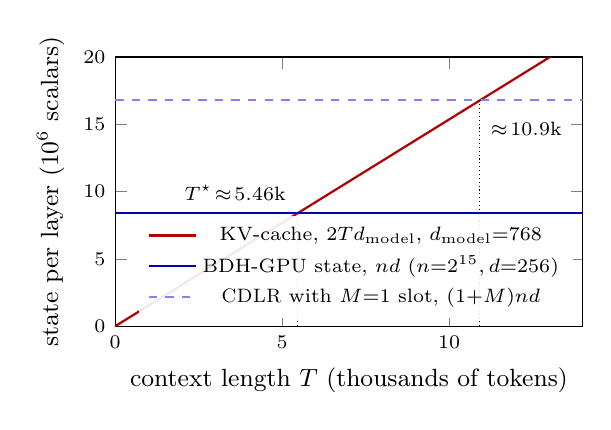
\begin{tikzpicture}
\begin{axis}[width=0.62\linewidth,height=5.0cm,
  xlabel={context length $T$ (thousands of tokens)},
  ylabel={state per layer ($10^6$ scalars)},
  xmin=0,xmax=14,ymin=0,ymax=20,
  legend style={font=\scriptsize,at={(0.98,0.03)},anchor=south east,draw=none,fill=white,fill opacity=0.9,text opacity=1},
  tick label style={font=\scriptsize},label style={font=\small}]
\addplot[thick,red!70!black,domain=0:14,samples=2]{1.536*x};
\addlegendentry{KV-cache, $2Td_{\text{model}}$, $d_{\text{model}}{=}768$}
\addplot[thick,blue!70!black,domain=0:14,samples=2]{8.389};
\addlegendentry{BDH-GPU state, $nd$ ($n{=}2^{15},d{=}256$)}
\addplot[thick,dashed,blue!50,domain=0:14,samples=2]{16.777};
\addlegendentry{\cdlr{} with $M{=}1$ slot, $(1{+}M)nd$}
\draw[densely dotted] (axis cs:5.461,0) -- (axis cs:5.461,8.389);
\node[font=\scriptsize,anchor=south east] at (axis cs:5.4,8.6) {$T^\star\!\approx\!5.46$k};
\draw[densely dotted] (axis cs:10.92,0) -- (axis cs:10.92,16.777);
\node[font=\scriptsize,anchor=north west] at (axis cs:10.95,15.9) {$\approx\!10.9$k};
\end{axis}
\end{tikzpicture}
\caption{Conceptual byte crossover from \cref{eq:crossover}. Lines are the closed-form state sizes, not
measurements. Each consolidated slot moves the crossover right by $T^\star$; the residual buffer $\mathcal{R}$ and
parameter bytes are omitted.}
\label{fig:crossover}
\end{figure}

\paragraph{Capacity.} Interference in a linear associative state grows with key overlap. BDH Claim~7 gives
$\tilde O(n)$ separable facts for non-adversarial keys and $\tilde\Omega(\sqrt n)$ in the worst case; to our
knowledge it has not been measured on recall benchmarks \citep{arora2023zoology}. This becomes H1 and E2.

\subsection{Single-timescale states couple retention and interference}
\label{sec:coupling}

Consider $\Sm_t=\lambda\Sm_{t-1}+u_t$, $0<\lambda<1$, with write $u_t$ (e.g.\ Hebbian $\phi(k_t)v_t^\top$). A stream
switches at $t_0$ from task $A$ (writes $u^A_t$) to task $B$ (writes $u^B_t$), both stationary in mean with means
$\bar u^A,\bar u^B$.

\begin{proposition}[Retention--interference coupling]
\label{prop:coupling}
At lag $\Delta\ge0$ after the switch, in expectation and in the stationary limit before $t_0$,
\[
\mathbb{E}\,\Sm_{t_0+\Delta}=\tfrac{1}{1-\lambda}\big(\lambda^{\Delta}\,\bar u^A+(1-\lambda^{\Delta})\,\bar u^B\big).
\]
The normalised weight of task $A$, $\alpha(\Delta)=\lambda^\Delta$, is simultaneously (i)~the \emph{retention} of
$A$ and (ii)~the \emph{interference} of $A$ with $B$-queries. With retention horizon
$H_{\mathrm{ret}}(\varepsilon)=\min\{\Delta:\alpha(\Delta)\le\varepsilon\}$ and adaptation horizon
$H_{\mathrm{ad}}(\delta)=\min\{\Delta:\alpha(\Delta)\le\delta\}$, for any $\lambda$,
$H_{\mathrm{ret}}(\varepsilon)/H_{\mathrm{ad}}(\delta)\to\log\varepsilon/\log\delta$, independent of $\lambda$.
In particular, if $A$ must stay retrievable ($\alpha\ge\varepsilon$) and $B$ uncontaminated ($\alpha\le\delta$) at the
same lag, with $\varepsilon>\delta$, no $\lambda$ satisfies both.
\end{proposition}
\begin{proof}
Unrolling, $\Sm_{t_0+\Delta}=\lambda^\Delta\Sm_{t_0}+\sum_{j=1}^{\Delta}\lambda^{\Delta-j}u^B_{t_0+j}$. In the
stationary limit $\mathbb{E}\Sm_{t_0}=\bar u^A/(1-\lambda)$, and $\sum_{j=1}^{\Delta}\lambda^{\Delta-j}=(1-\lambda^\Delta)/(1-\lambda)$,
which gives the expression. Both horizons solve $\lambda^\Delta=c$, i.e.\ $\Delta=\lceil\log c/\log\lambda\rceil$, so
their ratio tends to $\log\varepsilon/\log\delta$ (exactly, up to rounding), independent of $\lambda$. Requiring
$\lambda^\Delta\ge\varepsilon>\delta\ge\lambda^\Delta$ is a contradiction.
\end{proof}

\begin{remark}[Scope]
The statement concerns one shared, linearly superposed state. It does not rule out good continual behaviour for
(a)~input-dependent gates ($\lambda_t$ in Mamba/GLA/Gated DeltaNet), which can freeze the state but then also stop
adapting unless the gate infers task boundaries; (b)~delta rules, which remove interference along overwritten keys
but erase the overwritten association; (c)~high-dimensional sparse keys, which reduce overlap between $\bar u^A$ and
$\bar u^B$. Case (c) is BDH's implicit bet; it holds only while tasks occupy near-disjoint neurons, which the
language mixing of \citet[\S7.1]{kosowski2025bdh} suggests is not guaranteed. Cascade models
\citep{fusi2005cascade,benna2016consolidation} escape the coupling by adding variables with different time
constants; this is the design principle behind \cdlr.
\end{remark}

% ==================================================================
\section{Compact Dual-Timescale Latent Reasoning (\cdlr)}
\label{sec:method}

\cdlr{} is an architecture \emph{class}: the operator of \cref{def:amo} with both $\kappa$ and $\mathcal{F}$ present
and a hard byte budget (\cref{fig:cdlr}). Until E3 (with its byte-transfer control) and E4 are run, it is a design
and evaluation target, not a demonstrated method.

\begin{figure}[t]
\centering
\resizebox{0.92\linewidth}{!}{%
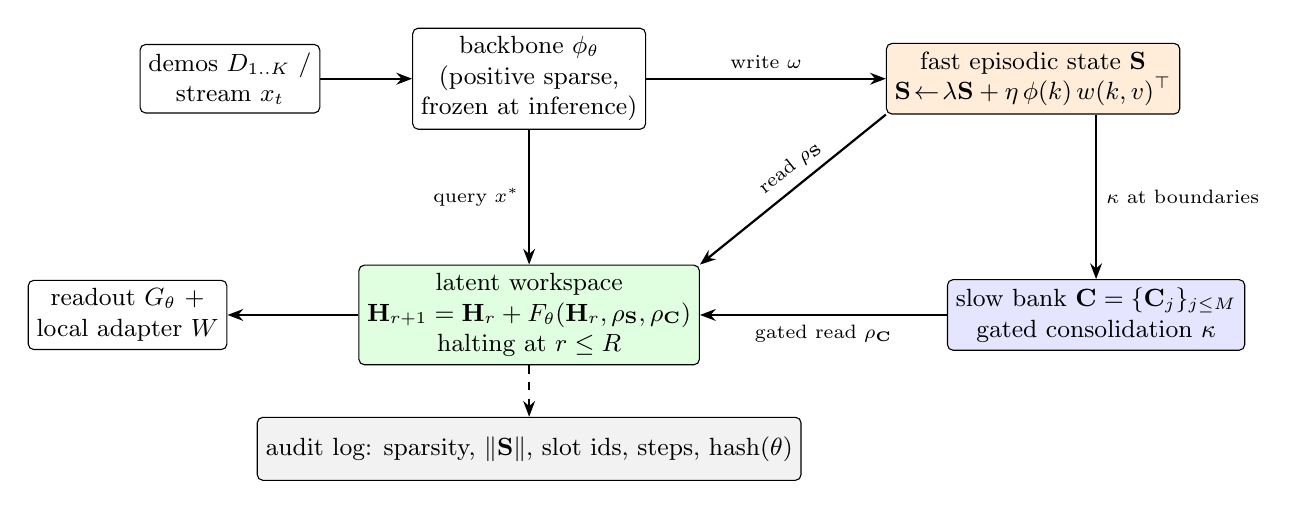
\begin{tikzpicture}[
  box/.style={draw,rounded corners=2pt,align=center,font=\small,minimum height=8mm,inner sep=3pt},
  fast/.style={box,fill=orange!15},
  slow/.style={box,fill=blue!10},
  ws/.style={box,fill=green!12},
  arr/.style={-{Stealth[length=2mm]},thick}]
\node[box] (in) at (-0.6,0) {demos $D_{1..K}$ /\\ stream $x_t$};
\node[box] (phi) at (3.2,0) {backbone $\phi_\theta$\\(positive sparse,\\ frozen at inference)};
\node[fast] (S) at (9.6,0) {fast episodic state $\Sm$\\$\Sm\!\leftarrow\!\lambda\Sm+\eta\,\phi(k)\,w(k,v)^\top$};
\node[ws] (H) at (3.2,-3.0) {latent workspace\\$\Hm_{r+1}=\Hm_r+F_\theta(\Hm_r,\rho_\Sm,\rho_\Cm)$\\halting at $r\le R$};
\node[slow] (C) at (10.4,-3.0) {slow bank $\Cm=\{\Cm_j\}_{j\le M}$\\gated consolidation $\kappa$};
\node[box] (G) at (-1.9,-3.0) {readout $G_\theta$ +\\local adapter $W$};
\node[box,fill=gray!10] (A) at (3.2,-4.7) {audit log: sparsity, $\|\Sm\|$, slot ids, steps, $\mathrm{hash}(\theta)$};
\draw[arr] (in) -- (phi);
\draw[arr] (phi) -- node[above,font=\scriptsize]{write $\omega$} (S);
\draw[arr] (S.south -| C.north) -- node[right,font=\scriptsize]{$\kappa$ at boundaries} (C.north);
\draw[arr] (S.south west) -- node[pos=0.45,above,sloped,font=\scriptsize]{read $\rho_\Sm$} (H.north east);
\draw[arr] (C) -- node[below,font=\scriptsize]{gated read $\rho_\Cm$} (H);
\draw[arr] (phi) -- node[left,font=\scriptsize]{query $x^*$} (H);
\draw[arr] (H) -- (G);
\draw[arr,dashed] (H) -- (A);
\end{tikzpicture}}
\caption{\cdlr{} data flow. Orange: fast timescale (within episode, decays). Blue: slow timescale (across episodes,
gated, not overwritten by an unmatched task). Green: latent workspace. Slow parameters $\theta$ are frozen at
inference; only $\Sm$, $\Cm$, and the optional adapter change, and the audit log records every change.}
\label{fig:cdlr}
\end{figure}

\paragraph{Backbone.} $\phi_\theta:\mathcal{X}\to\R^n_{\ge0}$ produces positive, sparse, high-dimensional codes. The
reference instantiation is a BDH-GPU stack (\citealp{kosowski2025bdh}, Def.~4) with k-winners-take-all and $\ell_2$
normalisation. A Transformer or SSM backbone with a positive projection head is a control that separates backbone
effects from memory-architecture effects.

\paragraph{Fast episodic state.} $\Sm\in\R^{n\times d_v}$ with normaliser $z\in\R^n$:
\begin{equation}
\Sm\leftarrow\lambda\Sm+\eta\,\phi(k)\,w_\theta(k,v)^\top,\qquad z\leftarrow\lambda z+\eta\,\phi(k),\qquad
\rho_\Sm(q)=\frac{\phi(q)^\top\Sm}{\phi(q)^\top z+\epsilon},
\label{eq:fast}
\end{equation}
with $\eta=\mathrm{softplus}(\cdot)$ and $\lambda=\mathrm{sigmoid}(\cdot)$ slow parameters. The delta-rule variant
$\Sm\leftarrow\lambda\Sm+\eta\,\phi(k)(w-\Sm^\top\phi(k))^\top$ \citep{schlag2021linear,yang2024deltanet} is a
first-class ablation because it changes the capacity regime of H1.

\paragraph{Slow consolidated bank and consolidation $\kappa$.} $\Cm=\{(\Cm_j,\mathbf{k}_j)\}_{j=1}^{M}$ holds at most
$M$ slots shaped like $\Sm$ (or rank-$r$ factorised), each with a summary key $\mathbf{k}_j$, plus a small reservoir
$\mathcal{R}$ of past codes for replay \citep{mcclelland1995cls}. At a consolidation event (episode boundary, or a
novelty trigger when the read error of $\Sm$ exceeds a threshold) we form
$\hat\Cm=\mathrm{unit}\big(\tfrac12\Sm+\tfrac12\,\Pi(\mathcal{R})\big)$, where $\Pi$ computes key-conditioned means of
replayed codes, and let $j^\star=\arg\max_j\cos(\hat\Cm,\Cm_j)$:
\begin{equation}
\kappa:\;\begin{cases}
\Cm_{j^\star}\leftarrow(1-\beta)\Cm_{j^\star}+\beta\hat\Cm & \text{if }\cos(\hat\Cm,\Cm_{j^\star})\ge\tau,\\
\text{allocate a new slot (evict least-used if }|\Cm|=M) & \text{otherwise.}
\end{cases}
\label{eq:consolidate}
\end{equation}
Reads are gated, $g_j=\mathrm{softmax}_j(\gamma s_j)$, with $s_j$ either key similarity
$\cos(\mathbf{k}_j,\bar\phi_{\text{ctx}})$ (unsupervised) or the fit of $\Cm_j$ to a labelled support set
(supervised; this leaks task information and must be reported as such); the term is dropped when
$\max_j s_j<\tau_{\text{gate}}$. Because $\Cm_j$ is written only when matched, task $A$'s slot is not diluted by
task $B$'s writes. This breaks the coupling of \cref{prop:coupling} at the cost of $M$ extra states and a
task-boundary or novelty signal.

\paragraph{Latent workspace.} Following BDH-CQ's public equations (\citealp{engdahl2026bdhcq}, Eqs.~2--4) with our
own open choices for every function:
\begin{align}
\Hm_0&=E_\theta\big(x^*,\rho_\Sm(\phi(x^*)),\textstyle\sum_jg_j\rho_{\Cm_j}(\phi(x^*))\big),\qquad
\Hm_{r+1}=\Hm_r+F_\theta\big([\Hm_r;\rho_\Sm(\kappa_k(W_q\Hm_r))]\big),\ r<R,\\
\hat y&=G_\theta(\Hm_{r^\star}),\quad r^\star=\min\{r:\max\mathrm{softmax}(G_\theta(\Hm_r))\ge c\}\wedge R,
\end{align}
where $\kappa_k$ is k-WTA and $c$ a halting threshold as in ACT \citep{graves2016act}. Every re-read uses the same
$\Sm$, so the workspace adds compute but no memory that grows with $R$.

\paragraph{Local adapter and audit.} An optional readout $W\phi+b$ adapts online by a three-factor rule
\citep{gerstner2018eligibility}, $e_t=\gamma e_{t-1}+\phi_t$, $W\mathrel{+}=\eta_W(y_t-p_t)e_t^\top$; nothing flows into
the backbone or back through time. For a linear head with $\gamma=0$ this is the cross-entropy gradient of that
head, so its locality lies in what it does \emph{not} touch; we do not claim it closes the no-BPTT gap of
\citet[\S7.2]{kosowski2025bdh}. Every \texttt{predict} call emits activation sparsity, $\|\Sm\|_F$, $\|\Delta\Hm\|$ per
step, halting step, selected slots and gates, consolidation actions, latency, and a hash of $\theta$ before and after,
turning ``no parameter updates at inference'' (\citealp{engdahl2026bdhcq}, \S1) into a checkable property. Slot-level
storage also allows targeted deletion of a consolidated episode.

\paragraph{Training and complexity.} Slow parameters are meta-trained on episodes with gradients through the $K$
within-episode writes, so \cdlr{} is \emph{not} BPTT-free during meta-training; at inference only $\Sm$, $\Cm$, and $W$
change. Per token and layer, a write and a read each cost $O(nd_v)$; the workspace adds $O(Rnd_v)$ per query and the
bank $O(|\{j:g_j>0\}|\,nd_v)$. Memory is $(1+M)nd_v b+|\mathcal{R}|nb$, constant in $T$ and in the number of past
episodes; \cref{eq:crossover} applies with $nd$ replaced by $(1+M)nd_v$ (\cref{fig:crossover}).

\paragraph{Falsifiable hypotheses.}
\begin{hypothesis}[Capacity]\label{h:cap}
At matched state bytes, recall accuracy of a positive, sparse, high-$n$ Hebbian state decays with the number of
stored pairs $N$ at a rate consistent with $\tilde O(n)$ capacity for random keys and degrades toward
$\tilde\Omega(\sqrt n)$ for correlated keys (BDH Claim~7). The delta variant beats the Hebbian variant on correlated keys.
\end{hypothesis}
\begin{hypothesis}[Dual timescale]\label{h:dual}
On interleaved task streams, \cdlr{} lowers forgetting relative to every single-state model with the same total
bytes, including input-gated SSMs, at no more than a fixed relative loss in plasticity. The gain disappears when the
bank is removed or its bytes are given to a larger $\Sm$.
\end{hypothesis}
\begin{hypothesis}[Workspace]\label{h:ws}
Latent iterations improve accuracy on compositional demonstration-conditioned tasks over $R=1$ at matched FLOPs, and
halting reduces mean compute without loss in accuracy.
\end{hypothesis}
\begin{hypothesis}[Where synaptic memory should lose]\label{h:lose}
On exact copying and high-cardinality multi-query recall at $T<T^\star$, softmax attention dominates every
bounded-state model on accuracy and on bytes. Reporting this region is part of the result.
\end{hypothesis}

% ==================================================================
\section{A Matched-Compute Evaluation Protocol}
\label{sec:protocol}

Claims about new architecture classes fail most often on accounting. Cost indicators disagree
\citep{dehghani2022efficiency}, and less-tuned baselines look worse, so we fix the protocol before running it; it is
frozen as a machine-readable preregistration in the supplementary material.

\paragraph{Principles.}
\textbf{P1 Matched budgets.} Non-embedding parameters, training tokens, and training FLOPs are matched within $\pm5\%$;
every comparison is run once matched on parameters and once on FLOPs, because BDH-GPU's $O(ndL)$ per-token cost
(\citealp{kosowski2025bdh}, \S4.2) and $3nd$ parameter count diverge from a Transformer's.
\textbf{P2 Equal tuning.} The same number of learning-rate/weight-decay sweep points per architecture; best and median of
sweep reported. \textbf{P3 Modern baselines.} Transformer++ (RoPE, SwiGLU, pre-norm), Mamba or Mamba-2, GLA or Gated
DeltaNet, plain linear attention at BDH's width, BDH-GPU from public code, and \cdlr; xLSTM and Titans where code
permits. \textbf{P4 Joint reporting.} Accuracy or loss; memory = parameter bytes + peak inference-state bytes at stated $T$
and batch; latency p50/p95 at batch~1 and saturated throughput on named hardware; results as Pareto fronts.
\textbf{P5 Statistics.} $\ge3$ seeds; Wilson intervals \citep{wilson1927probable}; exact McNemar \citep{mcnemar1947note} or
paired bootstrap; Holm correction. \textbf{P6 Preregistration and negative results.} H1--H4, metrics, and stopping rules
are frozen before runs; refuted hypotheses get the same prominence as confirmed ones. \textbf{P7 Reproducibility.}
Code, configs, seeds, logs, and audit records are released \citep{pineau2021reproducibility}; closed systems are
evaluated only as black boxes, and the paper says so.

\paragraph{E1. Language-modelling bakeoff beyond Europarl.} About 30M, 125M, and 350M non-embedding parameters at
${\sim}20$ tokens per parameter \citep{hoffmann2022chinchilla} on FineWeb-Edu \citep{penedo2024fineweb}, with a
Europarl byte-level replication \citep{koehn2005europarl} anchoring to \citet[App.~B.2]{kosowski2025bdh}. Outcomes:
loss-vs-FLOPs curves \citep{kaplan2020scaling}, a fixed zero-shot suite, and bytes/latency at
$T\in\{512,2\text{k},8\text{k},32\text{k}\}$, which brackets $T^\star$.

\paragraph{E2. Associative recall, capacity, and length generalisation (Claim~7, H1, H4).} Multi-query associative
recall \citep{arora2023zoology} with $N$ swept until failure at $n\in\{2^{12},\dots,2^{16}\}$ and matched state bytes.
Keys i.i.d.\ and with controlled correlation. We fit $N_{50}(n)$, the $N$ at 50\% recall, and test whether its
exponent is near 1 (random keys) or $\tfrac12$ (correlated keys). Length generalisation: train at $T$, test at
$2T$--$16T$ on recall, copying \citep{jelassi2024repeat}, and RULER-style needles \citep{hsieh2024ruler}, with BDH's
damping ablated.

\paragraph{E3. Ablation ladder (\cref{fig:ladder}).} Each rung adds one component at fixed bytes and FLOPs, from
plain linear attention to full \cdlr. A \emph{byte-transfer control} at rung (g) gives the bank's bytes to a larger
$\Sm$, so ``more memory'' and ``a second timescale'' are not confounded; a \emph{backbone control} replaces BDH with
a Transformer plus positive head.

\begin{figure}[t]
\centering
\resizebox{\linewidth}{!}{%
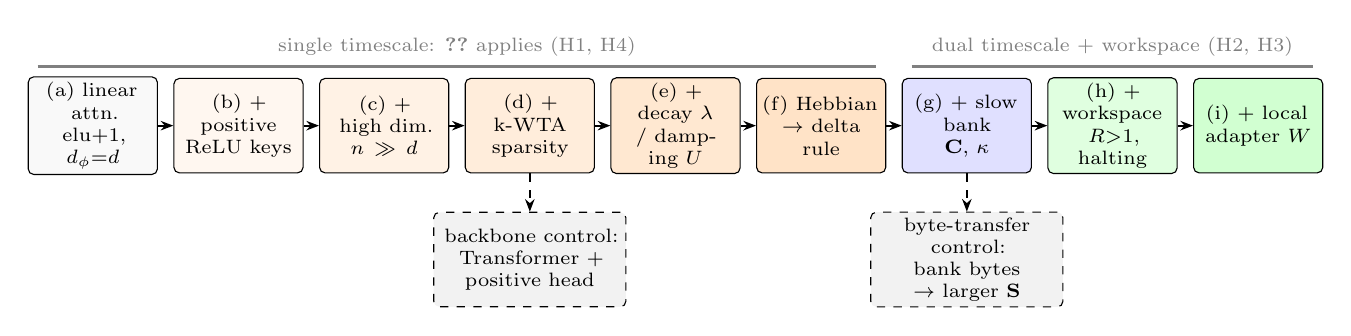
\begin{tikzpicture}[
  rung/.style={draw,rounded corners=2pt,align=center,font=\scriptsize,minimum height=12mm,text width=1.5cm,inner sep=2pt},
  ctrl/.style={rung,dashed,fill=gray!10,text width=2.3cm},
  arr/.style={-{Stealth[length=1.6mm]},thick}]
\node[rung,fill=gray!5]  (a) at (0,0)    {(a) linear attn.\\elu$+1$, $d_\phi{=}d$};
\node[rung,fill=orange!6] (b) at (1.85,0) {(b) $+$ positive\\ReLU keys};
\node[rung,fill=orange!10](c) at (3.7,0)  {(c) $+$ high dim.\\$n\gg d$};
\node[rung,fill=orange!14](d) at (5.55,0) {(d) $+$ k-WTA\\sparsity};
\node[rung,fill=orange!18](e) at (7.4,0)  {(e) $+$ decay $\lambda$\\/ damping $U$};
\node[rung,fill=orange!22](f) at (9.25,0) {(f) Hebbian\\$\to$ delta rule};
\node[rung,fill=blue!12]  (g) at (11.1,0) {(g) $+$ slow bank\\$\Cm$, $\kappa$};
\node[rung,fill=green!12] (h) at (12.95,0){(h) $+$ workspace\\$R{>}1$, halting};
\node[rung,fill=green!18] (i) at (14.8,0) {(i) $+$ local\\adapter $W$};
\foreach \u/\v in {a/b,b/c,c/d,d/e,e/f,f/g,g/h,h/i} \draw[arr] (\u) -- (\v);
\node[ctrl] (bt) at (11.1,-1.7) {byte-transfer control:\\bank bytes $\to$ larger $\Sm$};
\node[ctrl] (bb) at (5.55,-1.7) {backbone control:\\Transformer $+$ positive head};
\draw[arr,dashed] (g) -- (bt);
\draw[arr,dashed] (d) -- (bb);
\draw[decorate,thick,gray] (-0.7,0.75) -- (9.95,0.75) node[midway,above,font=\scriptsize]{single timescale: \cref{prop:coupling} applies (H1, H4)};
\draw[decorate,thick,gray] (10.4,0.75) -- (15.5,0.75) node[midway,above,font=\scriptsize]{dual timescale $+$ workspace (H2, H3)};
\end{tikzpicture}}
\caption{Conceptual E3 ablation ladder. Each rung changes one component at fixed state bytes and FLOPs; dashed boxes
are controls. The diagram defines the experiment; it reports no results.}
\label{fig:ladder}
\end{figure}

\paragraph{E4. Continual streams (H2).} Streams $A\!\to\!B\!\to\!A\!\to\!\dots$ with controlled interference: permuted
mappings, class-incremental symbol tasks, and language-domain streams. Metrics: average accuracy, forgetting,
backward and forward transfer \citep{lopezpaz2017gem}, relearning speed, plasticity loss \citep{dohare2024loss}, and
total bytes. Baselines: frozen, full fine-tuning, replay \citep{rolnick2019replay}, EWC \citep{kirkpatrick2017ewc}, a
fast-state-only model, and input-gated SSMs, each with and without task-boundary signals.

\paragraph{E5. Demonstration-conditioned latent reasoning (H3).} ARC-AGI-1 public evaluation, ConceptARC
\citep{moskvichev2023conceptarc}, and RE-ARC controls \citep{hodel2024rearc}, with no evaluation tasks or task
identifiers in training (\citealp{engdahl2026bdhcq}, \S1). BDH-CQ appears only as (i)~its \emph{reported} numbers or a
black-box run if access is granted, or (ii)~a \emph{clearly labelled reimplementation} of its Eqs.~1--4
(``BDH-CQ-R''). Contamination controls use disjoint hashes and a freshly authored held-out set; cost per task is
reported under an explicit accounting (GPU type, seconds, price, pipeline stages).

\paragraph{Compute envelope.} At $6ND$ FLOPs the E1 grid (30M/0.6B, 125M/2.5B, 350M/7B tokens) costs
${\approx}1.7\times10^{19}$ FLOPs per architecture-seed, or ${\approx}2.5\times10^{20}$ for five architectures and three
seeds: about 550 A100-hours at 40\% utilisation (${\approx}1.1$k with sweeps). E2--E4 are an order of magnitude cheaper.

% ==================================================================
\section{Critical Analysis of BDH and BDH-CQ}
\label{sec:critique}

Both papers make real contributions. BDH gives an explicit bridge from attention to local synaptic dynamics, with a
clear parameter count, public code, and testable theory. BDH-CQ reports an independent black-box audit that reproduced
its 29.5\% pass@2 without weight access (\citealp{engdahl2026bdhcq}, \S5), byte-identical repeat runs (\S6.6), Wilson
intervals, and candid failure analyses (\S6.2--6.4). Our critique concerns what the evidence licenses
(\cref{tab:critique}).

\begin{table}[t]
\centering
\scriptsize
\caption{Claims, evidence, and gaps. \PS: paper-stated limitation; \IN: our inference.}
\label{tab:critique}
\begin{tabularx}{\linewidth}{@{}>{\raggedright\arraybackslash}p{3.3cm}>{\raggedright\arraybackslash}X>{\raggedright\arraybackslash}X@{}}
\toprule
Claim (source) & Evidence reported & Gap \\
\midrule
BDH rivals GPT-2 at 10M--1B params (\citealp{kosowski2025bdh}, Abstract; \S4.2, Fig.~7) &
Europarl En--Pl/En--Cs byte-level, 1.2B tokens; GPTXL baseline (nanoGPT + Transformer-XL buffer + ALiBi), App.~B.2, Table~4 &
\IN{} One corpus family; values graphical only; no modern linear/SSM baselines in experiments though cited (\S4.3); no FLOP-matched curve.\\
Monosemantic synapses (\S6.3) & Mann--Whitney $U=2368$, $p<10^{-14}$, 50+50 LLM-generated sentences, one concept pair, one layer &
\IN{} Single concept pair; no comparison with SAE features in Transformers \citep{bricken2023monosemanticity}.\\
Capacity $\tilde O(n)$ / $\tilde\Omega(\sqrt n)$ (Claim~7, \S6.1, App.~C.2) & Proof sketch (JL + Azuma) &
\IN{} Not measured on recall benchmarks; motivates E2.\\
Reasoning generalises over length/time (\S1) & -- &
\PS{} Thermodynamic-limit/PAC-like bounds are a goal (Abstract, \S1). \IN{} Not directly tested.\\
Long context, no hard bound (\S6.1) & -- & \PS{} Damping (RoPE+ALiBi-like) still required.\\
Model merging by concatenation in $n$ (\S7.1, Table~2) & Merged 38M model, X$\to$En loss 0.39--0.43 &
\PS{} Merged model mixes languages when translating from English.\\
Training without BPTT (\S7.2) & English loss $\approx0.65\to0.75$--$1.05$ & \PS{} Degradation; cross-language concept matching lost.\\
Sparse/neuromorphic execution (\S2.4) & Cost estimate & \PS{} CPU sparse kernels $10^2$--$10^5\times$ less cost-effective than GPU BDH-GPU. \IN{} Energy not measured.\\
\midrule
BDH-CQ 29.5\% pass@2 ARC-AGI-1, \$0.00070/task (\citealp{engdahl2026bdhcq}, Abstract; \S5, Table~1) &
118/400, Wilson [25.24, 34.15]; $\approx$0.85 H200 GPU-s at \$3/h; independent black-box audit &
\IN{} \S6.6 prices STANDARD effort (also 118/400) at \$0.00265246/task and MIN at \$0.00088399; relation to the \$0.00070 headline not stated.\\
Architecture & ``Dimensions, exact update rules, and implementation details remain proprietary'' (\S3.3); recipe proprietary (\S4.1) &
\PS{} Not reproducible from text. \IN{} No ablation separating BDH backbone from candidate construction/ranking.\\
Generalisation to ConceptARC (\S6.1, Table~1) & 95/160 semantic, 96/160 opaque pass@2 &
\PS{} ConceptARC is in the training mixture (\S4.2); exposure via training or checkpoint selection not ruled out (\S6.5).\\
pass@2 semantics (\S6.6) & 75 single-candidate records & \PS{} pass@2 is not two independent attempts for every input.\\
Compositional boundaries (\S6.2--6.3, App.~A.3) & Ordering 1/24 at length 8; colour swap 0/72 composed; conditional rule selection 100\%$\to$56.7\% &
\PS{} Stated weaknesses. Ladders are single-family, 40 tasks (App.~A.4); mechanic rates confounded by LLM authoring (App.~A.2).\\
Scaling ``1B to 600B'' (\S9.2) & No figure, table, or numbers & \IN{} Unsupported by reported data.\\
\bottomrule
\end{tabularx}
\end{table}

\paragraph{Open problems.} (1)~\emph{Measured capacity}: does BDH-GPU's high-$n$ positive state reach Claim~7's regime,
and beat gated/delta models at equal \emph{bytes}? (E2) (2)~\emph{Which ingredient matters}: positivity, sparsity,
high $n$, weight sharing, or damping? No published experiment isolates these. (E3) (3)~\emph{Interference}: merging by
concatenation and continual adaptation both need a mechanism that keeps tasks apart, which decay alone cannot provide
(\cref{prop:coupling}; E4). (4)~\emph{Latent reasoning without a proprietary pipeline}: how much ARC performance survives
an open reimplementation of Eqs.~1--4? (E5) (5)~\emph{Cost accounting}: cost-per-task frontiers need one published
accounting of hardware, pipeline stages, and effort tier.

% ==================================================================
\section{Discussion}
\label{sec:discussion}

\paragraph{Why a dual timescale.} Softmax attention avoids the plasticity--stability dilemma by never forgetting within
the window and never learning across windows. Fixed-state models learn online but share one state, so by
\cref{prop:coupling} they trade retention against interference. Weight-level continual learning
\citep{kirkpatrick2017ewc,zenke2017si} works on the slowest timescale and needs gradients. \cdlr{} adds the missing
inference-time timescale, by analogy with hippocampal-to-neocortical transfer \citep{mcclelland1995cls} and
multi-timescale synapses \citep{benna2016consolidation}, while memory stays bounded and slow weights stay frozen. H2 is
falsifiable, and E3's byte-transfer control is designed to refute it if it is wrong.

\paragraph{Where \cdlr{} should lose.} We hold H4 as likely: below $T^\star$, and on exact copying or high-cardinality
recall \citep{arora2023zoology,jelassi2024repeat}, a KV-cache is both smaller and more accurate. A hybrid of local
softmax attention plus \cdlr{} memory is the natural compromise and belongs in E1--E2. Bank selection needs a
task-boundary/novelty signal or a labelled support set, and the unsupervised gate may fail where tasks share inputs.

\paragraph{Limitations.} (i)~No large-scale results are reported; the protocol's cost is stated above.
(ii)~\Cref{prop:coupling} is a linear, expected-value statement; nonlinear readouts and input-dependent gates need a
richer analysis. (iii)~\cdlr{} adds hyperparameters ($M,\tau,\beta,\gamma,R,c$) that could absorb tuning budget, hence
P2. (iv)~Meta-training uses BPTT across demonstrations. (v)~The BDH-CQ audit relies on its text alone, because the
system is closed. (vi)~Positive sparse codes and slot-structured memory give audit signals (which neurons wrote,
which slot was read, how many steps ran), not explanations.

% ==================================================================
\section{Conclusion}
\label{sec:conclusion}

Softmax attention, Hebbian synaptic state, and recurrent latent memory are three settings of one associative-memory
operator, differing in growth, key geometry, forgetting, consolidation, and workspace. This view yields a closed-form
memory crossover, exposes retention--interference coupling in any single-timescale state, and motivates \cdlr, a fast
episodic state plus a slow gated bank with a latent workspace and an audit trail. We separated what BDH and BDH-CQ
state from what we infer, and specified a matched-compute protocol under which they and \cdlr{} can be confirmed or
refuted, including the cases where the KV-cache wins.

\section*{Broader Impact Statement}
Models that learn at inference change behaviour after deployment. This raises the risk of memory poisoning through
crafted demonstrations, by analogy with training-time poisoning \citep{wallace2021poisoning}, and the risk that
consolidated slots retain personal data. The \cdlr{} audit log, parameter hash, and slot-level deletion are partial
mitigations that make writes visible and reversible; deployments should cap consolidation rates, require provenance
for consolidated episodes, and support rollback. Bounded-memory inference can lower serving energy for long contexts,
but only above $T^\star$, and this should be measured, not assumed.

\paragraph{Code availability.} An anonymized archive with the protocol code, configurations, the frozen
preregistration (\texttt{prereg/e1\_e5\_protocol\_v0.json}), and smoke-test logs is provided as supplementary
material; a public repository link will be added in the camera-ready version.

\bibliography{references}
\bibliographystyle{tmlr}

% ==================================================================
\appendix
\section{Preliminary Smoke Tests (Not Main Results)}
\label{app:probes}

\textbf{Status.} Single-machine CPU runs on synthetic toy tasks with $5\times10^4$ to $1.6\times10^6$ parameters. They
check that the protocol and audit pipeline run end to end and illustrate what mismatched budgets do. They provide
\emph{no} evidence about the hypotheses at scale, about ARC, or about the BDH \S7.2 gap. Numbers come from run files
in the supplementary archive (seed and date in the logs).

\paragraph{P1: Episodic write without weight change (Tiny-\cdlr, 52,531 params).} BDH backbone (public
\texttt{bdh.py}, unchanged, $n_{\text{embd}}{=}32$, 2 layers, 256 sparse units), $K{=}4$ demonstrations per episode on a
random key$\to$value map with 16 classes (chance 0.0625). Accuracy with demonstrations written into $\Sm$ was 1.00,
vs.\ 0.086 for the same queries with an empty $\Sm$. The parameter hash was identical before and after inference.
Mean halting step was 1.23 of $R{=}3$.

\paragraph{P2: A$\to$B$\to$A with full interference.} A and B are different permutations of the same 16 inputs. A
fast-state-only arm forgot A completely after B (A accuracy $1.00\to0.00$; first-5 relearning accuracy 0.04). The
dual-timescale arm kept A at 1.00 (first-5 relearning 0.80). \emph{Caveat:} slot selection used a labelled 32-token
support set at evaluation, which is a task-identity signal, so this probe does not test the unsupervised gate.

\paragraph{P3: Local adapter vs.\ BPTT (negative result).} On a lag-1 permutation stream over a small pretrained BDH
(3 seeds, 150 steps/phase), a local delta-rule readout with fast Oja memory reached 0.81 average online accuracy vs.\
0.91 for full BPTT, at about $2.3\times$ lower per-step cost. \emph{Both forgot task A almost completely} (forgetting gap
0.97 in both), as \cref{prop:coupling} predicts for a single shared state.

\paragraph{P4: Why matched budgets matter.} A 300-step Shakespeare character run had BDH reach validation loss 1.875 vs.\
2.43--2.44 for a Transformer and a linear-attention model, but BDH had $1.9\times$ the parameters (1.64M vs.\ 0.87M),
took $12\times$ the wall time, and the baselines were still on an early plateau: the comparison is not matched and
supports no ranking. In a toy Tiny-\cdlr{} vs.\ Transformer recall comparison, the undertrained Transformer was far less
accurate (0.25 vs.\ 1.00) but $28\times$ faster and used less memory at this context length.

\section{Reporting Checklist for Architecture Bakeoffs}
\label{app:checklist}
\begin{enumerate}[leftmargin=*,itemsep=0pt]
\item Non-embedding params, training tokens, training FLOPs (method stated), wall time, hardware.
\item Sweep grid and size per architecture; best and median of sweep.
\item Inference bytes: parameters + state at each reported $T$ and batch; latency p50/p95; throughput.
\item Seeds, intervals, paired tests, multiple-comparison correction.
\item Data provenance and contamination checks (hash overlap) for every evaluation set.
\item For closed systems: black-box status, access date, and exactly which numbers are quoted.
\item Preregistered hypotheses with outcome (confirmed / refuted / inconclusive).
\end{enumerate}

\section{Notation}
\label{app:notation}
\begin{tabular}{@{}ll@{}}
$T$ & sequence length (tokens)\\
$n$ & neuron dimension (BDH) / key-feature dimension\\
$d,d_v,d_{\text{model}}$ & low-rank width, value width, Transformer width\\
$\Sm,z$ & fast episodic state and normaliser\\
$\Cm_j,\mathbf{k}_j,M$ & slow bank slot, slot key, slot budget\\
$\lambda,\eta$ & fast decay, fast write rate\\
$\kappa,\beta,\tau$ & consolidation map, merge rate, merge threshold\\
$\Hm_r,R,c$ & workspace state, max steps, halting confidence\\
$T^\star$ & byte crossover between KV-cache and bounded state (\cref{eq:crossover})\\
\end{tabular}

\end{document}
